\documentclass[a4paper,14pt]{extarticle}
\usepackage[utf8]{inputenc}
\usepackage[russian]{babel}
\usepackage{graphicx}
\usepackage{indentfirst}
\usepackage[top=0.8in, bottom=0.8in, left=0.8in, right=0.8in]{geometry}
\usepackage{pgfplots}
\usepackage{amsmath}
\usepackage{setspace}
\usepackage{titlesec}
\usepackage{subcaption}
\usepackage{float}
\usepackage{chngcntr}
\usepackage{pgfplots}
\usepackage{amsfonts}
\usepackage{hhline}
\usepackage{pgfplotstable}
\usepackage{multirow}
\usepackage{karnaugh-map}
\usepackage{tikz,xcolor}

\titleformat{\section}[hang]
  {\bfseries}
  {}
  {0em}
  {\hspace{-0.4pt}\large \thesection\hspace{0.6em}}
  
  
\titleformat{\subsection}[hang]
  {\bfseries}
  {}
  {0em}
  {\hspace{-0.4pt}\large \thesubsection\hspace{0.6em}}

%\linespread{1.3} % полуторный интервал
%\renewcommand{\rmdefault}{ftm} % Times New Roman

\newcommand{\nx}{\overline{x}}
\newcommand{\p}{0.31}
\newcommand{\scale}{1.4}

\counterwithin{figure}{section}
\counterwithin{equation}{section}
\counterwithin{table}{section}

\begin{document}
\begin{titlepage}
\centering
Санкт-Петербургский политехнический университет Петра Великого \\
Институт компьютерных наук и технологий \\
Кафедра компьютерных систем и программных технологий \\
\vspace{6.0cm}

{\centering \textbf{Отчёт по лабораторным работам} \\ 
\vspace{0.15cm}
\textbf{Дисциплина}: Телекоммуникационные технологии} \\

\vspace{6.8cm}

\begin{table}[H]
\begin{tabular}{p{\textwidth}@{}r}
{Выполнил студент гр. 33501/4} \hfill { $\underset{\text{(подпись)}}{\underline{\hspace{0.23\textwidth}}}$ Жуйков А.А.} \\
{Преподаватель} \hfill { $\underset{\text{(подпись)}}{\underline{\hspace{0.23\textwidth}}}~~~~$ Богач Н.В.} \\
\vspace{0.15cm}
{} \hfill { <<\underline{\hspace{0.08\textwidth}}>> \underline{\hspace{0.2\textwidth}}2018 г.} \\
\end{tabular}
\end{table}
\vfill
{\centering Санкт-Петербург \\ 
\vspace{0.15cm}
2018}
\end{titlepage}

\section{Лабораторная работа №1. Сигналы телекоммуникационных систем.}
\subsection{Цель работы.}
Познакомиться со средствами генерации и визуализации простых сигналов.

\subsection{Постановка задачи.}
В командном окне MATLAB и в среде Simulink промоделировать синусоидальный и прямоугольный сигналы с различными параметрами. Получить их спектры. Вывести на график.

\subsection{Теоретические положения.}
\subsubsection{Классификация сигналов.}
Сигнал – это носитель информации, используемый для передачи сообщений в системе связи. Чаще всего он рассматривается как зависимость напряжения от времени.

Сигналы делятся на \textit{дискретные} и \textit{непрерывные}. В случае, когда параметр сигнала принимает последовательное во времени конечное число значений, сигнал называется дискретным. Непрерывный сигнал принимает множество значений из некоторого диапазона. Между значениями, которые он принимает, нет разрывов.

Сигнал может быть \textit{периодическим} или \textit{непериодическим}. К периодическим относят гармонические и полигармонические сигналы. Для периодических сигналов выполняется общее условие:
\begin{equation*}
s(t) = s(t + kT),
\end{equation*}
где $k$ = 1, 2, 3, ... -- любое целое число, $T$ -- период, являющийся конечным отрезком независимой переменной. К непериодическим сигналам относят почти периодические и апериодические сигналы. Основным инструментом их анализа является частотное представление.

По длительности сигналы делятся на \textit{бесконечные} и \textit{конечные (финитные)}. Финитные сигналы — это сигналы конечной длительности, т.е. существующие на конечном временном интервале. Они отличны от нуля на этом интервале и равны нулю за его пределами.

\textit{Дельта-функция} $\delta(t)$, или \textit{функция Дирака}, представляет собой бесконечно узкий импульс с бесконечной амплитудой, расположенный при
нулевом значении аргумента функции:
\begin{equation*}
\delta(t) = \begin{cases} 0, & t \neq 0; \\ \infty, & t = 0. \end{cases}
\end{equation*}
При этом выполняется соотношение:
\begin{equation*}
\int_{-\infty}^\infty \delta(t)dt = 1.
\end{equation*}
Несмотря на физическую нереализуемость, дельта-функция играет значительную роль для теоретического анализа сигналов и систем. Одно из важных свойств функции Дирака -- это фильтрующее свойство:
\begin{equation*}
\int_A^B f(t) \delta(t - t_0) dt = \begin{cases} f(t_0), & t_0 \in [A, B]; \\ 0, & t_0 \notin [A, B], \end{cases}.
\end{equation*}
где пределы $A$ и $B$ могут быть бесконечными.

\subsubsection{Ряд Фурье. Прямое и обратное преобразование Фурье.}
Разложению в \textit{ряд Фурье} могут подвергаться периодические сигна-
лы. При этом они представляются в виде суммы гармонических функций ли-
бо комплексных экспонент с частотами, образующими арифметическую про-
грессию. Для того чтобы такое разложение существовало, фрагмент сигнала
длительностью в один период должен удовлетворять условиям Дирихле:
\begin{itemize}
\item не должно быть разрывов 2-ого рода;
\item число разрывов 1-ого рода должно быть конечно;
\item число экстремумов должно быть конечным.
\end{itemize}
Для непериодических сигналов разложение в ряд Фурье неприменимо,
но эта проблема решается путем предельного перехода в предположении, что
сигнал имеет период, стремящийся к бесконечности.

В синусно-косинусной форме ряд Фурье имеет следующий вид:
\begin{equation}
s(t) = \frac{a_0}{2} + \sum_{k=1}^\infty (a_k \cos(k\omega t) + b_k \sin(k\omega t)).
\label{ddd}
\end{equation}
Коэффициенты $a_k$ и $b_k$ рассчитываются по формулам:
\begin{equation*}
a_k = \frac{2}{T} \int_{-T/2}^{T/2} s(t) \cos (k\omega t) dt,
\end{equation*}
\begin{equation*}
a_k = \frac{2}{T} \int_{-T/2}^{T/2} s(t) \sin (k\omega t) dt,
\end{equation*}

Применив к формуле \ref{ddd} тригонометрические преобразования, можно
заменить сумму синуса и косинуса на косинус той же частоты с иной амплитудой и некоторый начальной фазой. В результате получается вещественная форма ряда Фурье:
\begin{equation*}
s(t) = \frac{a_0}{2} + \sum_{k=1}^\infty A_k \cos(k\omega t + \varphi_k),
\end{equation*}
где $A_k = \sqrt{a_k^2 + b_k^2}$, $\varphi = \arctan(b_k/a_k)$.

Наиболее часто в радиотехнике употребляется комплексная форма ряда Фурье:
\begin{equation*}
\cos (x) = \frac{1}{2} (e^{jx} + e^{-jx}).
\end{equation*}

Совокупность амплитуд гармоник ряда Фурье часто называют амплитудным спектром, а совокупность фаз – фазовым спектром. \\

\textit{Преобразование Фурье} -- это инструмент спектрального анализа непериодических сигналов. 

Переход от ряда Фурье к преобразованию Фурье осуществляется путем устремления периода сигнала к бесконечности. При этом гармоники в ряду Фурье располагаются настолько плотно, что делают спектр непрерывным. Результатом вычислений является функция частоты $S(\omega)$ -- \textit{спектральная функция} сигнала $s(t)$. Формула \textit{преобразования Фурье}:
\begin{equation*}
S(\omega) = \int_{-\infty}^{\infty} s(t)e^{-j\omega t} dt.
\end{equation*}
\textit{Обратное преобразование Фурье:}
\begin{equation*}
s(t) = \frac{1}{2\pi} \int_{-\infty}^{\infty} S(\omega)e^{j\omega t} d\omega.
\end{equation*}
При использовании частоты $f$ формулы принимают вид:
\begin{equation*}
S(f) = \int_{-\infty}^{\infty} s(t)e^{-j2\pi ft} dt ~~\text{и} ~~ s(t) = \int_{-\infty}^\infty S(f) e^{j2\pi ft} df.
\end{equation*}
Модуль спектральной функции называют амплитудным спектром, а её аргумент -- фазовым спектром.

Таким образом, преобразование Фурье ставит в соответствие сигналу,
заданному во времени, его спектральную функцию. При этом говорят, то осуществляется \textit{переход из временной области в частотную}. Преобразование Фурье взаимно-однозначно, поэтому представление сигнала в частотной области (спектральная функция) содержит столько же информации, сколько и исходный сигнал, заданный во временной области.

\subsection{Ход работы.}
\subsubsection{Прямоугольный импульс.}
Единичный прямоугольный импульс, центрированный относительно начала отсчета времени, с амплитудой A и длительностью T можно представить выражением:
\begin{equation*}
s(t) = \begin{cases} A, & |t| \leq T/2 \\ 0, & |t| > T/2 \end{cases}
\end{equation*}
Ниже на Рис. \ref{rect} приведен импульс с амплитудой 1 и длительностью 0.2, полученный в Matlab. На Рис. \ref{rect_} представлен спектр данного импульса.
\begin{figure}[H]
\centering
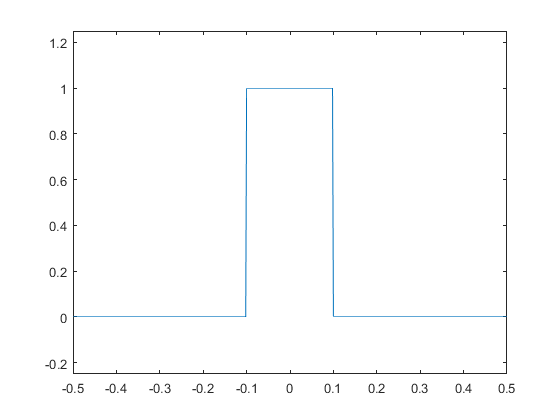
\includegraphics[scale=0.75]{pics/1rect.png}
\caption{Единичный прямоугольный импульс.}
\label{rect}
\end{figure}

\begin{figure}[H]
\centering
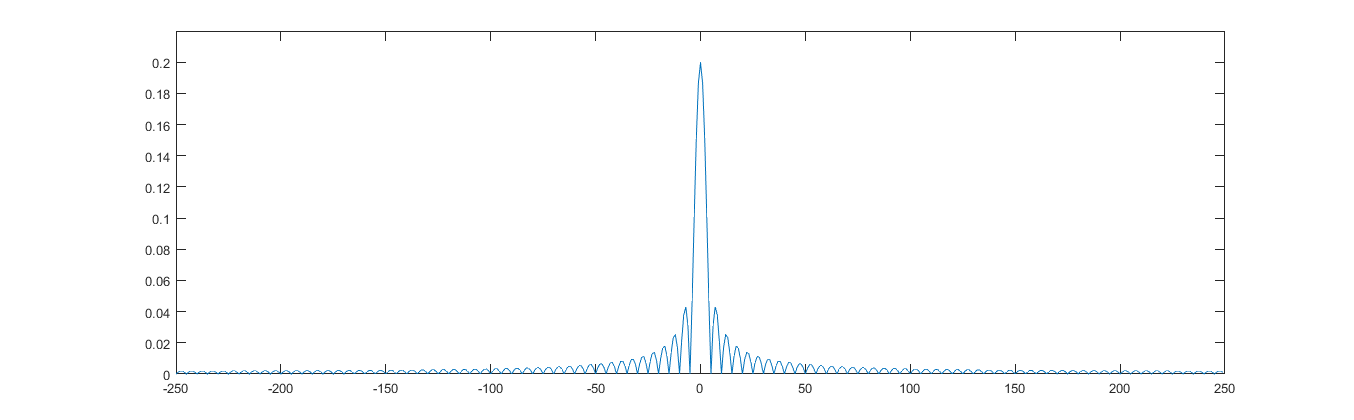
\includegraphics[scale=0.5]{pics/1rect_spec.png}
\caption{Спектр единичного прямоугольного импульса.}
\label{rect_}
\end{figure}

\subsubsection{Гармонический сигнал.}
Одним из наиболее часто используемых типов периодических сигналов является гармоническое колебание, описываемое уравнением $s (t) = A sin (\omega_0 t + \varphi_0 )$, где A – амплитуда, $\omega_0 = 2 \pi f_0$ – круговая частота, $\varphi_0$ – начальная фаза. Величина $(\omega_0 t + \varphi_0)$ определяет полную фазу сигнала. Таким образом, гармоническое колебание полностью характеризуется тремя параметрами: частотой (или периодом), амплитудой и фазой.

В Matlab был получен синусоидальный сигнал с различной частотой: 5 Гц (Рис. \ref{sin5}), 100 Гц (Рис. \ref{sin100}) и 500 Гц. На Рис. \ref{sin5_} -- \ref{sin500_} представлены спектры этих сигналов.

\begin{figure}[H]
\centering
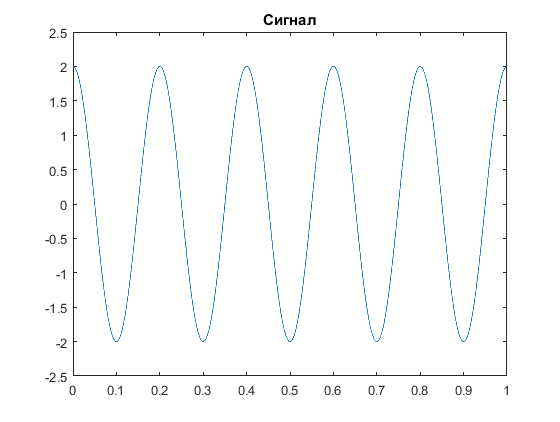
\includegraphics[scale=0.75]{pics/1sin5Hz.png}
\caption{Синусоидальный сигнал. $f_0$ = 5 Гц.}
\label{sin5}
\end{figure}
\begin{figure}[H]
\centering
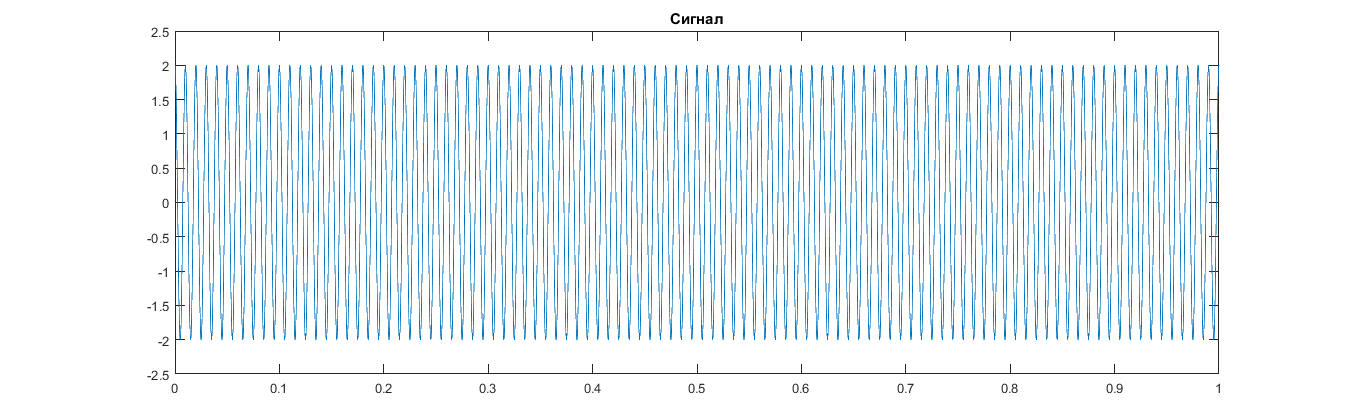
\includegraphics[scale=0.5]{pics/1sin100Hz.png}
\caption{Синусоидальный сигнал. $f_0$ = 100 Гц.}
\label{sin100}
\end{figure}
\begin{figure}[H]
\centering
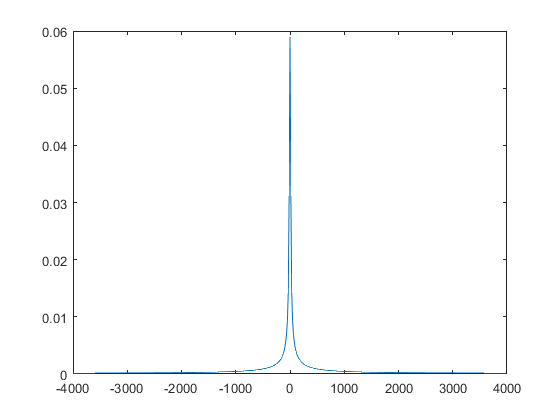
\includegraphics[scale=0.75]{pics/1sin5Hz_spec.png}
\caption{Спектр синусоидального сигнала. $f_0$ = 5 Гц.}
\label{sin5_}
\end{figure}
\begin{figure}[H]
\centering
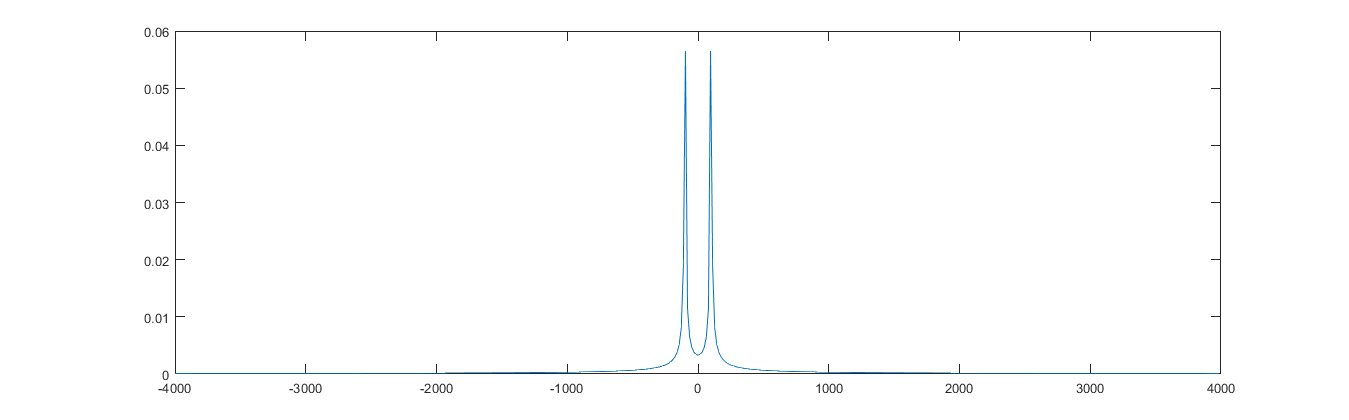
\includegraphics[scale=0.5]{pics/1sin100Hz_spec.png}
\caption{Спектр синусоидального сигнала. $f_0$ = 100 Гц.}
\label{sin100_}
\end{figure}
\begin{figure}[H]
\centering
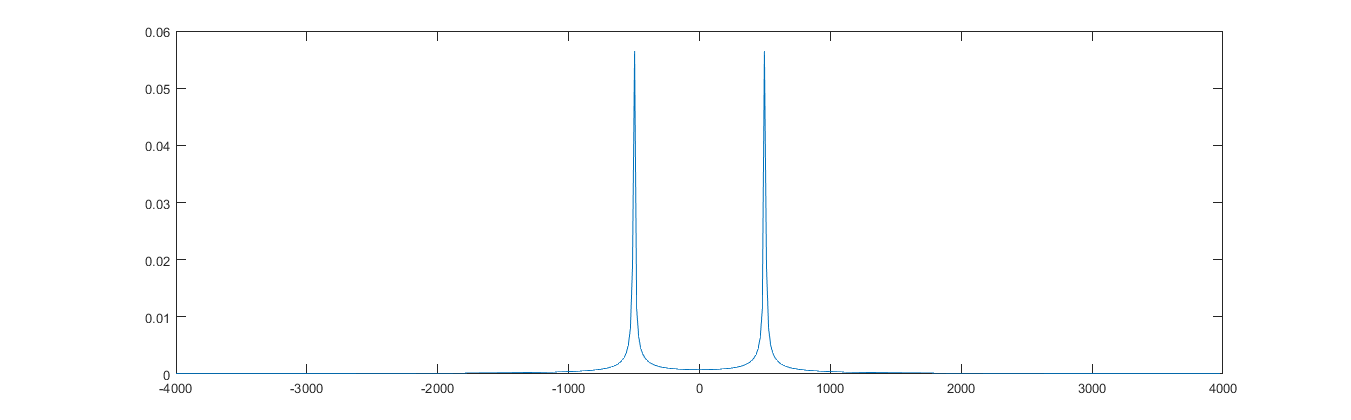
\includegraphics[scale=0.5]{pics/1sin500Hz_spec.png}
\caption{Спектр синусоидального сигнала. $f_0$ = 500 Гц.}
\label{sin500_}
\end{figure}

\subsubsection{Треугольный сигнал.}
Треугольный периодический сигнал с частотой 10 Гц представлен на Рис. \ref{treug}. Спектр сигнала приведен на Рис. \ref{treug_}.
\begin{figure}[H]
\centering
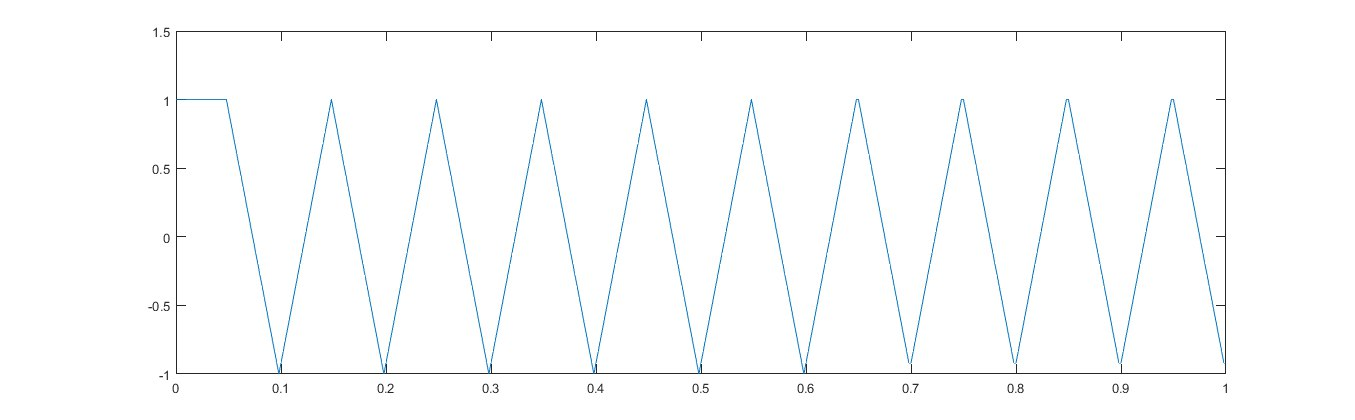
\includegraphics[scale=0.5]{pics/1treug.jpg}
\caption{Треугольный периодический сигнал.}
\label{treug}
\end{figure}
\begin{figure}[H]
\centering
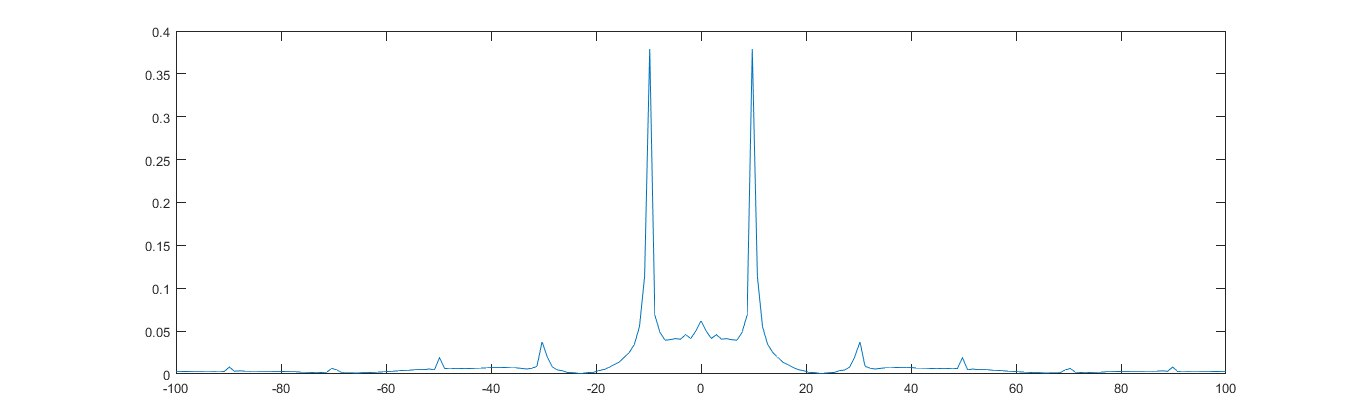
\includegraphics[scale=0.5]{pics/1treug_spec.jpg}
\caption{Спектр треугольного периодического сигнала.}
\label{treug_}
\end{figure}

\subsubsection{Сигнал с меняющейся частотой.}
C помощью функции Matlab \textit{chirp} был получен сигнал с меняющейся частотой. График полученного сигнала представлен на Рис. \ref{chirp}. Видно, как частота  сигнала меняется от низких значений до высоких линейно во времени. Спектр сигнала представлен на Рис. \ref{chirp_}.
\begin{figure}[H]
\centering
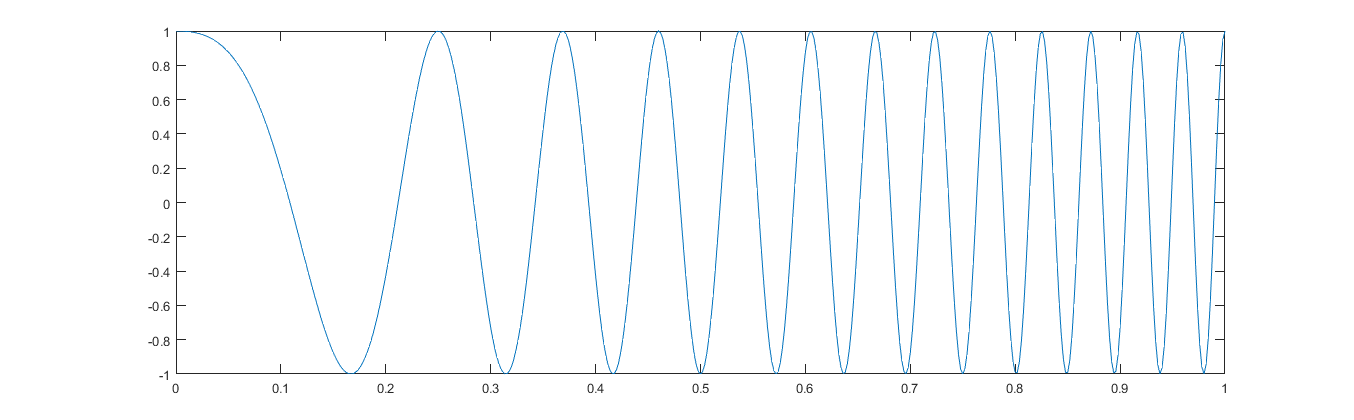
\includegraphics[scale=0.5]{pics/1chirp.png}
\caption{Сигнал с меняющейся частотой.}
\label{chirp}
\end{figure}
\begin{figure}[H]
\centering
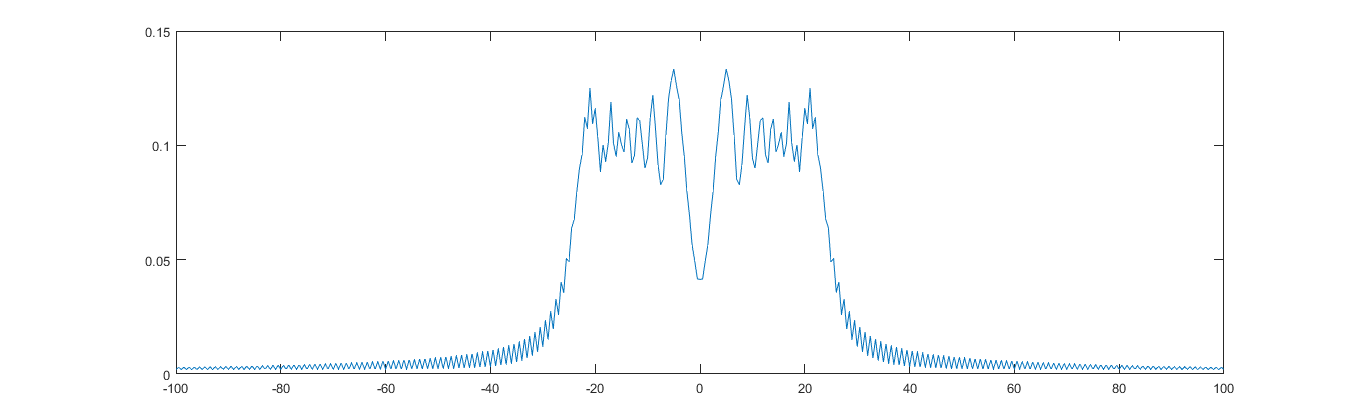
\includegraphics[scale=0.5]{pics/1chirp_spec.png}
\caption{Спектр сигнала с меняющейся частотой.}
\label{chirp_}
\end{figure}

\subsubsection{Моделирование сигнала в среде Simulink.}
В среде Simulink, интегрированой в Matlab, было проведено моделирование сигнала, а также получение его спектра. Для генерации сигнала был использован элемент \textit{Sine Wave}; его настройки приведены на Рис. \ref{sine_wave}. Для наблюдения сигнала использован элемент \textit{Scope}. Полученная схема предсталена на Рис. \ref{scheme}.
\begin{figure}[H]
\centering
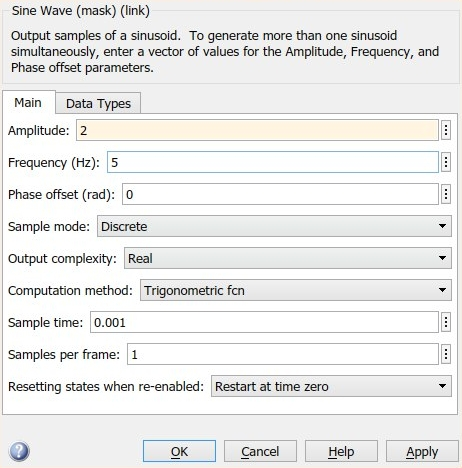
\includegraphics[scale=0.5]{pics/1simulink_params.jpg}
\caption{Параметры Sine Wave.}
\label{sine_wave}
\end{figure}
\begin{figure}[H]
\centering
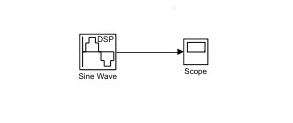
\includegraphics[scale=1.2]{pics/1simulink_scheme.jpg}
\caption{Схема для наблюдения сигнала в среде Simulink.}
\label{scheme}
\end{figure}

Сигнал, полученный с помощью элемента \textit{Scope}, представлен на Рис. \ref{simulink_signal}. Для получения спектра данного сигнала использован элемент \textit{Spectrum Analyzer}. Спектр представлен на Рис. \ref{simulink_signal_}.
\begin{figure}[H]
\centering
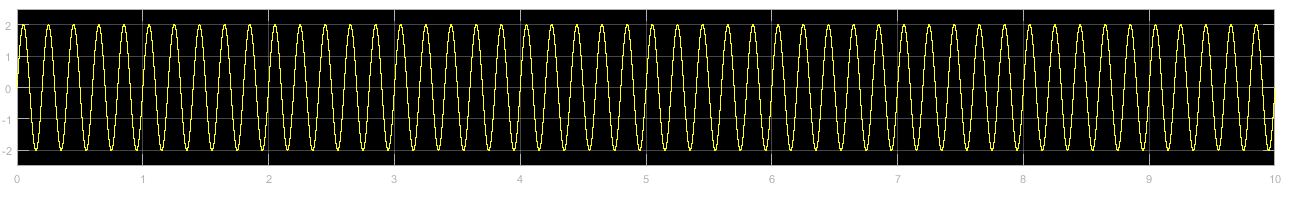
\includegraphics[scale=0.5]{pics/1simulink_001.png}
\caption{Сигнал, полученный в среде Simulink.}
\label{simulink_signal}
\end{figure}
\begin{figure}[H]
\centering
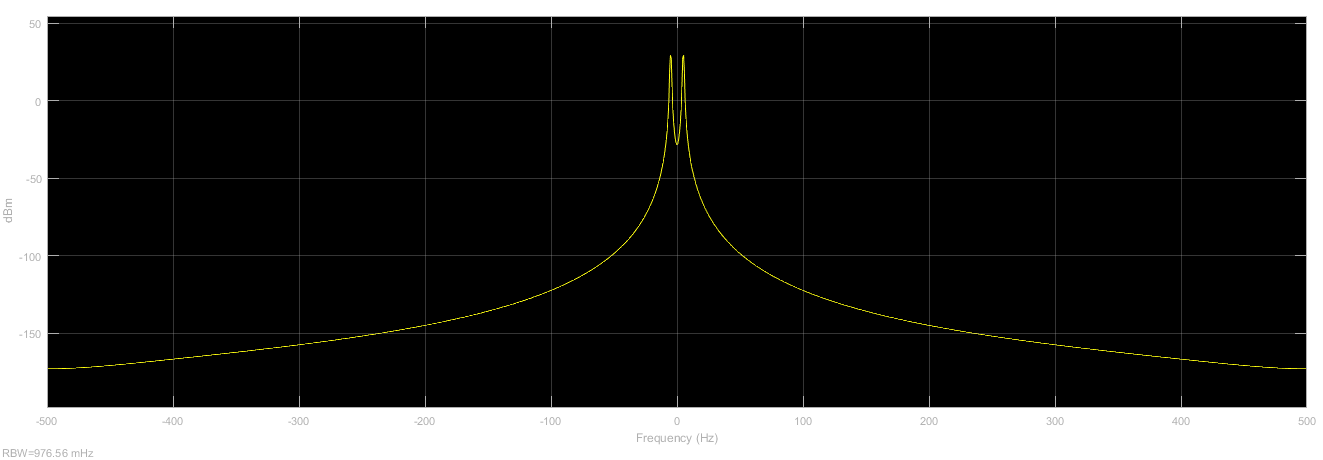
\includegraphics[scale=0.5]{pics/1simulink_spec.png}
\caption{Спектр сигнала, полученный в Simulink.}
\label{simulink_signal_}
\end{figure}

\subsection{Выводы}
Сигналы используются для передачи информации. Они классифицируются по различным признакам: \textit{периодические} и \textit{непереодические}; \textit{дискретные} и \textit{непрерывные}; \textit{бесконечные} и \textit{конечные}.

Сигнал может быть представлен как во временной, так и в частотной области (спектр сигнала). При этом выполняются свойства:
\begin{itemize}
\setlength\itemsep{0.1cm}
\item Дискретный сигнал имеет периодический спектр.
\item Периодический сигнал имеет дискретный спектр.
\item Ограниченный во времени сигнал имеет бесконечный спектр.
\end{itemize}

В результаты лабораторной работы функциями языка Matlab, а также средствами среды Simulink были сгенерированы и визуализированы сигналы с различными характеристиками, получены их спектры.

\newpage % <<<<<<-----------------------------------------------------


\section{Лабораторная работа №2. Корреляция.}
\subsection{Цель работы.}
Получить представление о спектрах телекоммуникационных сигналов.

\subsection{Постановка задачи.}
\begin{itemize}
\item Для сигналов, построенных в лабораторной работе №1, выполните расчет преобразования Фурье. Перечислите свойства
преобразования Фурье.
\item С помощью функции корреляции найдите позицию синхропосылки [101] в сигнале [0001010111000010]. Получите пакет
данных, если известно, что его длина составляет 8 бит без
учета синхропосылки. Вычислите корреляцию прямым методом, воспользуйтесь алгоритмом быстрой корреляции, сравните время работы обоих алгоритмов.
\end{itemize}

\subsection{Теоретические положения.}
\subsubsection{Свойства преобразования Фурье.}
Под свойствами преобразования Фурье (см. лаб. работу №1) подразумевается взаимное соответствие трансформаций сигналов и их спектров. Преобразование Фурье обладает следующими свойствами:
\begin{itemize}
\item[1.] \textit{Линейность.} Спектр линейной комбинации сигналов есть линейная комбинация спектров этих сигналов.
\item[2.] \textit{Задержка.} Если исходный сигнал получает задержку $\tau$, то его спектральная функция умножается на $e^{-j\omega \tau}$ . На практике это означает, что амплитудный спектр остается неизменным, а фазовый -- приобретает
дополнительное слагаемое $-\omega \tau$ (линейно зависящее от частоты).
\item[3.] \textit{Масштабирование по времени.} Изменение длительности сигнала в $a$ раз приводит к изменению ширины его спектра в противоположную сторону в сочетании с увеличением (при растяжении, |$a$| < 1) или уменьшением (при сжатии, |$a$| > 1) уровня спектральных составляющих. Если
$a$ < 0, происходит зеркальное отражение спектра относительно нулевой
частоты.
\item[4.] \textit{Дифференцирование сигнала.} Спектр производной получается путем умножения исходного спектра на $j \omega$, что соответствует ослаблению
низких частот и усилению высоких. Фазовый спектр при этом сдвигается на 90 градусов для $\omega$ > 0 и на $-90$ градусов для $\omega$ < 0.
\item[5.] \textit{Интегрирование сигнала.} Если исходный сигнал $f (t)$ не содержит постоянной составляющей, то есть выполняется равенство
$$\int^{\infty}_{-\infty} f(t) dt = 0,$$ то спектр его интеграла равен спектру исходного сигнала, деленного на $j \omega$. Если же соотношение не выполняется, то в общем случае результат выглядит следующим образом:
$$S(\omega) = \frac{F(\omega)}{j\omega} + \pi F(0)\delta(\omega)$$ при интегрировании исходного сигнала высокие частоты ослабляются, а низкие усиливаются. Фазовый спектр смещается на -90 градусов для
$\omega$ > 0 и на 90 градусов для $\omega$ < 0.
\item[6.] \textit{Спектр свертки сигналов.} Спектр свертки сигналов равен произведению спектров этих сигналов.
\item[7.] \textit{Спектр произведения сигналов.} Спектр произведения сигналов представляет собой свертку их спектров, деленную на 2$\pi$.
\item[8.] \textit{Умножение сигнала на гармоническую функцию.} Если исходный
сигнал умножить на гармоническую функцию, то его спектр распадется
на два слагаемых, одинаково смещенных на величину частоты гармонического колебания влево и вправо по отношению к исходному спектру, а уровни спектральных составляющих уменьшатся вдвое и будут
умножены на величину, учитывающую начальную фазу гармонического колебания.
\end{itemize}


\subsubsection{Корреляция сигналов.}
Для измерения степени сходства двух сигналов применяют понятие
\textit{корреляции}. В дискретном случае взаимная корреляция (cross-correlation) двух сигналов вычисляется по формуле:
\begin{equation*}
r_{12}(i) = \frac{1}{N} \sum^{N-1}_{n=0} x_2(n)x_1(n+i),
\end{equation*}
где $n$ = 0...$N-1$ -- временные отчеты, $i$ -- задержка, т.е. число отсчетов,
на которые сигнал $x_2(n)$ отстает от сигнала $x_1 (n)$.

Для определения взаимосвязи сигналов корреляция должна быть вычислена для различных значений задержек. Наибольшее значение корреляции считается истинным.

В непрерывной временной области функция взаимной корреляции для
периодических сигналов с периодом T определяется как
\begin{equation*}
r_{12}(\tau) = \frac{1}{T} \int^T_0 x_1(t) x_2(t + \tau) dt,
\end{equation*}
а для сигналов конечной длительности как 
\begin{equation*}
r_{12}(\tau) = \int^{\infty}_{-\infty} x_1(t) x_2(t + \tau) dt.
\end{equation*}

Расчет корреляции можно ускорить, используя теорему о корреляции:
\begin{equation*}
r_{12} = \frac{1}{N} \mathcal{F}_D^{-1} [\overline{X_1}(k)X_2(k)],
\end{equation*}
где $X_1(k) = \mathcal{F}_D [x_1(n)],~ X_2(k) = \mathcal{F}_D[x_2(n)]$, $\mathcal{F}_D[...], \mathcal{F}_D^{-1}[...]$ -- прямое и
обратное дискретные преобразования Фурье (ДПФ) соответственно, которые
обычно вычисляются с использованием алгоритма быстрого преобразования
Фурье (БПФ). Если число членов в последовательностях $x_1 (n)$ и $x_2(n)$ достаточно велико, то данный метод, называемый \textit{быстрой корреляцией}, дает результат быстрее, чем непосредственный расчет взаимной корреляции.

\subsection{Ход работы.}
\subsubsection{Вычисление кросс-корреляции.}
Имеется синхропосылка [1 0 1] и сигнал [0 0 0 1 0 1 0 1 1 1 0 0 0 0 1 0]. С помощью функций xcorr и ifft в MATLAB была вычислена кросс-корреляция и быстрая корреляция соответственно. В результате получены графики, приведенные на Рис. \ref{2graph1} и Рис. \ref{2graph2}.
\begin{figure}[H]
\centering
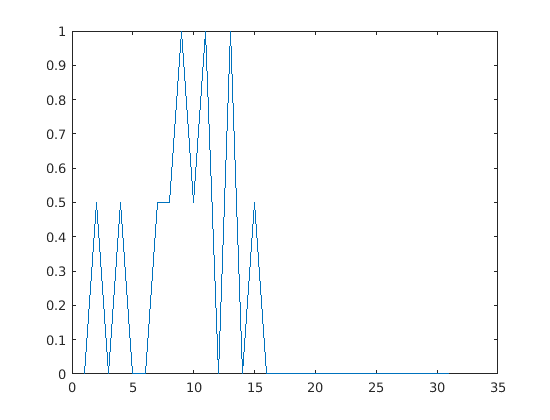
\includegraphics[scale=0.7]{pics/2corr.png}
\caption{Результаты вычисления кросс-корреляции функцией xcorr.}
\label{2graph1}
\centering
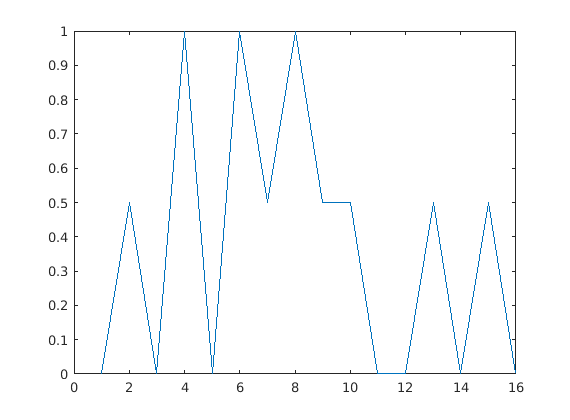
\includegraphics[scale=0.7]{pics/2corr2.png}
\caption{Результаты вычисления быстрой кросс-корреляции функцией ifft.}
\label{2graph2}
\end{figure}

При этом время вычислений при расчете кросс-корреляции оказалось следующим:
\begin{figure}[H]
\centering
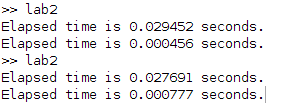
\includegraphics[scale=0.9]{pics/2elapsed.png}
\caption{Время вычисления кросс-корреляции.}
\end{figure}
\textit{Примечание:} в первой строке вывода указано время вычисления кросс-корреляции функцией xcorr, во второй -- функцией ifft. Видно, что алгоритм быстрой корреляции справился с задачей в среднем в 50 раз быстрее.

\subsubsection{Сравнение времени выполнения алгоритов вычисления кросс-корреляции}
Сравнение времени выполнения алгоритов вычисления кросс-корреляции выполнялось для следующей синхропосылки: [1 0 1]. Сигнал представлял собой случайную последовательность нулей и единиц различной длины в пределах от 15 бит до 8 млн бит. Результаты представлены в таблице \ref{2table}, а также на Рис. \ref{2graph_}.
\begin{figure}[H]
\centering
\begin{tikzpicture}
\begin{axis}[
%	ylabel near ticks,
%	xlabel near ticks,
	legend pos=north west,
    height = 0.4\textheight,
    width=0.8\textwidth,
	xlabel={№п/п},
	ylabel={$t$, с},
	%ylabel style={rotate=-90},
	xticklabel style={/pgf/number format/.cd,fixed,precision=2}
]
\addplot table [x=step, y=xcorr, col sep=comma] {data.csv};
\addplot table [x=step, y=ifft, col sep=comma] {data.csv};
\legend{xcorr, ifft};
\end{axis}
\end{tikzpicture} \hfill
\caption{График зависимости $t_{xcorr}$, $t_{ifft}$ от $N_\text{сигнала}$.}
\label{2graph_}
\end{figure}

\begin{table}[H]
\centering
\caption{Зависимость $t_{xcorr}$, $t_{ifft}$ от $N_\text{сигнала}$.}
\pgfplotstabletypeset[col sep=comma,
    columns={step, len, xcorr, ifft},
    column type/.add={|c|}{},
    columns/step/.style={ column name={№п/п}},
    columns/len/.style={column name={Длина сигнала}, int detect},
    columns/xcorr/.style={ column name={$t_{xcorr}$, с}, precision=9},
    columns/ifft/.style={ column name={$t_{ifft}$, с}, sci zerofill, precision=9},
    every nth row={1}{before row=\hline},
    every head row/.style = {before row=\hline, after row=\hline},
    every last row/.style = {after row=\hline},
   ]{data.csv}
   \label{2table}
\end{table}

Таким образом, с увеличением длины посылки время работы функции xcorr увеличивается быстрее, чем время работы функции вычисления быстрой корреляции ifft. 

\subsection{Вывод.}
Преобразование Фурье имеет широкое применение в телекоммуникационных технологиях. Оно позволяет совершать переход из временной области в частотную и наоборот. Некоторые свойства сигналов сложно выявить, рассматривая их во времени, в то время как их частотное представление позволяет легко определить ряд параметров.

В качестве примера можно привести задачу выделения гармонических
составляющих в зашумленном сигнале. Если амплитуда шумов сравнима с
амплитудой сигнала, то, рассматривая его временную диаграмму, сложно различить сигнал и шум. При построении спектра сигнала, гармоники будут хорошо видны полосы частот, занятой шумами.

Корреляция сигналов играет значительную роль в обработке сигналов. Она используется при решении задач идентификации сигналов в шуме, двоичных кодовых слов в системе с импульсно-кодовой модуляцией и других областях. Корреляцию можно найти по определению, а также с помощью алгоримта быстрой корреляции (алгоритм ускорен с помощью быстрого преобразования Фурье). В ходе эксперимента было выявлено, что вычисление быстрой корреляцией, не зависимо от длины сигнала, позволяет получить результат быстрее, чем вычисление по определению. 

\end{document}
